\documentclass[dvipsnames, svgnames, x11names, a4paper, 11pt]{article}

% URLs and hyperlinks ------------------------------
\usepackage{hyperref}
\hypersetup{
    colorlinks=true,
    linkcolor=NavyBlue,
    filecolor=magenta,      
    urlcolor=blue,
}
\usepackage{xurl}
%---------------------------------------------------

\usepackage{float}
\usepackage{graphicx}
\usepackage{listings}
\usepackage{color}
\usepackage{xcolor}

\definecolor{dkgreen}{rgb}{0,0.6,0}
\definecolor{gray}{rgb}{0.5,0.5,0.5}
\definecolor{mauve}{rgb}{0.58,0,0.82}

\lstset{frame=tb,
    language=vhdl,
    aboveskip=3mm,
    belowskip=3mm,
    showstringspaces=false,
    columns=flexible,
    basicstyle=\ttfamily,
    numbers=left,
    numberstyle=\small\color{gray},
    keywordstyle=\bfseries\color{Green4},
    commentstyle=\color{gray},
    stringstyle=\color{mauve},
    breaklines=true,
    breakatwhitespace=true,
    tabsize=4,
    identifierstyle=\color{black}
}

\usepackage{xepersian}
\settextfont{Yas}

\title{حافظه‌های \lr{ROM} و \lr{BRAM}}
\author{
فاطمه علی‌ملکی \\
مهدی حق‌وردی
}

\begin{document}
\maketitle
\tableofcontents

\section{توضیحات فایل‌های تمرین}
\subsection{فایل \lr{\texttt{rom8x8}}}
این فایل، ساده‌ترین فایل این تمرین است که شامل یک موجودیت به نام
\lr{\texttt{rom8x8}}
و یک معماری به نام 
\lr{\texttt{behave}}
است.

\subsubsection{توضیحات موجودیت \lr{\texttt{rom8x8}}}
این موجودیت شامل دو پورت است:
\begin{itemize}
\item 
\lr{\texttt{addr}}

این پورت یک ورودی 
\lr{\texttt{std\_logic\_vector}} 
۳ بیتی است که در واقع مقدار خروجی را تعیین می‌کند.

\item 
\lr{\texttt{dout}}

این پورت هم یک پورت خروجی از نوع 
\lr{\texttt{std\_logic\_vector}}
۸ بیتی است که مقدار خروجی روی آن قرار می‌گیرد.
\end{itemize}

\subsubsection{توضیحات معماری \lr{\texttt{behave}}}
این تنها معماری حاضر برای موجودیت 
\lr{\texttt{rom8x8}}
است که در واقع یک \lr{decoder} ۳ به ۸ است.

مقادیری که برای خروجی انتخاب شده‌اند کاملا \lr{hard code} شده‌اند و این کاملا با نام موجودیت (که \lr{\texttt{rom}} است) هماهنگی دارد.

در معماری از 
\lr{language feature}
عی به نام 
\lr{\texttt{with ... select}}
استفاده شده است که با توجه به مقدار 
\lr{\texttt{addr}}
خروجی را روی 
\lr{\texttt{dout}}
قرار می‌دهد.

\subsection{فایل \lr{romram}}
این فایل در واقع کل پروژه و کد این شکل است:
\begin{figure}[H]
\begin{center}
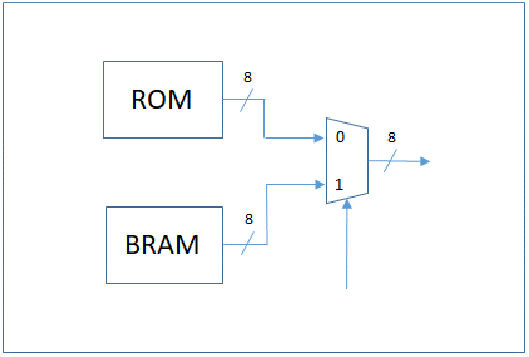
\includegraphics[width=0.7\textwidth, height=0.3\textheight]{images/project}
\end{center}
\end{figure}
چرا کد این شکل است؟

چون در کد مشاهده‌ می‌شود که مشخصا موجودیت‌های 
\lr{\texttt{rom8x8}}
،
\lr{\texttt{clock\_divide}}
و
\lr{\texttt{bram8x8}}
در آن به عنوان یک 
\lr{component}
استفاده شده‌اند (که موجودیت‌هایی هستند که در شکل وجود دارند، البته مالتی پلکسری که در شکل است در قسمت معماری همین فایل تعریف شده است).

کد شامل یک موجودیت به نام
\lr{\texttt{romram}}
و یک معماری به نام
\lr{\texttt{structural}}
است.

\subsubsection{موجودیت \lr{\texttt{romram}}}
موجودیت دارای دو ورودی و یک خروجی‌ست:
\begin{itemize}
\item 
ورودی‌ها

\begin{itemize}
\item \lr{\texttt{clk\_100MHZ}}

از نوع 
\lr{\texttt{std\_logic}}
و تبعا یک بیتی‌ست که کلاک سیستم است.

\item  \lr{\texttt{switch}}

از نوع 
\lr{\texttt{std\_logic}}
است که همان پایه‌ی انتخاب داخل شکل پروژه است.

\end{itemize}

\item 
خروجی
\begin{itemize}
\item \lr{\texttt{leds}}

یک پورت ۸ بیتی از نوع 
\lr{\texttt{std\_logic\_vector}}
است مقداری انتخاب شده روی آن قرار می‌گیرد.

\end{itemize}

\end{itemize}

\subsubsection{معماری \lr{\texttt{structural}}}
در قسمت معماری این فایل، ابتدا ۳ 
\lr{component}ی 
که در این پروژه استفاده شده‌اند، تعریف شده‌اند و پس از آن ۵ سینگال میانی تعریف و مقداردهی اولیه شده‌اند.
 
در قسمت \lr{\texttt{begin}} این معماری، ابتدا ۳ \lr{component} بالا اصطلاحا 
\lr{\texttt{port map}}
شده و به سینگال‌های ورودی، میانی و خروجی وصل شده‌اند.

معماری شامل یک \lr{\texttt{process}} است که به سیگنال 
\lr{\texttt{clk\_1Hz}}
حساس است. سپس این فرآیند برای هر یک کلاک با مقدار ۱، با توجه به ورودی \lr{\texttt{switch}} که ۰ باشد یا ۱، خروجی را به ترتیب با 
\lr{\texttt{dout\_rom}}
و یا
\lr{\texttt{dout\_bram}}
پر می‌کند. سپس فارغ از مقدار \lr{\texttt{switch}} یک شمارنده یا یکی اضافه می‌کند.
\subsection{فایل \lr{clockDivider}}
شامل یک موجودیت و یک معماری‌ست:
\subsubsection{موجودیت \lr{\texttt{clock\_divide}}}
صرفا شامل یک ورودی و یک خروجی یک بیتی به نام‌های 
\lr{\texttt{clk\_in}}
و 
\lr{\texttt{clk\_out}}
است.

\subsubsection{معماری \lr{\texttt{behave}}}
این معماری شامل ۴ سینگال میانی و سه فرآیند است.

\begin{itemize}
\item 
سیگنال‌های میانی

شامل دو سینگال از نوع
\lr{\texttt{unsigned}} 
به طول ۲۷ بیت، و دو سینگال یک بیتی از نوع 
\lr{\texttt{std\_logic}}
است.

\item 
فرآیند‌ها

قسمت معماری این فایل شامل ۳ فرايند و یک 
\lr{statement}
است که به صورت موازی اجرا می‌شوند.

کلاکی که بورد پازج در اختیار ما قرار می‌دهد، کلاک 
\lr{100MHz}
است که چشم انسان قابلیت دیدن تغییرات آن را روی چیزی مانند \lr{LED} ندارد.

برای تبدیل کردن این تعداد کلاک بسیار زیاد به یک کلاک در ثانیه می‌توان تا نصف این عدد را مقدار صفر داد و نصف دیگر را عدد یک. این فایل‌ هم دقیقا همین کار را انجام می‌دهد. این فایل دونه دونه کلاک‌ها را می‌شمارد و یک متغیر را با هر کلاک یکی اضافه می‌کند، تا زمانی که به مقدار 
\lr{50e6}
که نصف 
\lr{100MHz}
است برسد؛ و تا این زمان، سیگنالی که روی خروجی می‌افتد را 
\lr{\texttt{(oeb\_next)}}
صفر می‌کند.

از بعد از عدد 
\lr{50e6}
به همین منوال، سیگنال
\lr{\texttt{oeb\_next}}
مقدار ۱ را داراست.
\end{itemize}

\section{تغییرات کد برای بلوک دیاگرام}
بلوک دیاگرامی که در گروه فرستادید، تغییراتی را در کد 
\lr{\texttt{romram.vhd}}
می‌طلبید که تغییرات آن با استفاده از پلاگین \lr{git} نرم‌افزار 
\lr{PyCharm Community Edition}
عکس گرفته شده‌اند.

\subsection{ورودی‌ها}
تغییرات کلی ورودی‌‌‌ها در تصویر 
\ref{fig:input-changes}
آورده شده‌اند.

\subsection{}

\begin{figure}[b]
\begin{center}
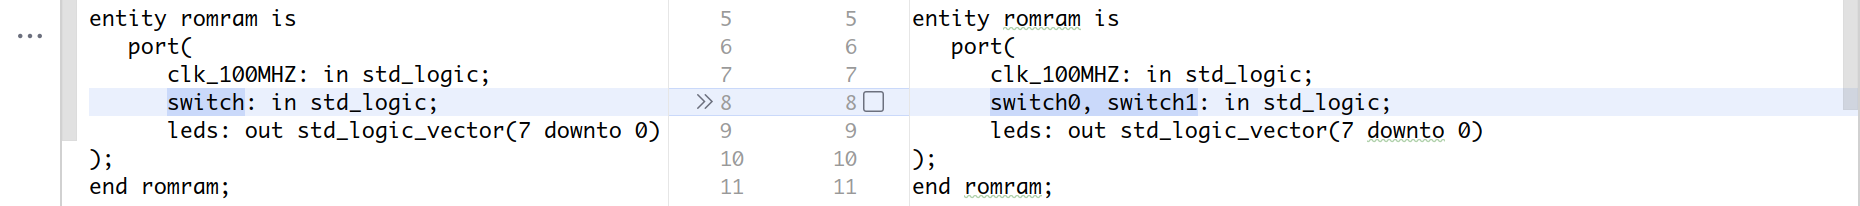
\includegraphics[width=0.90\textheight, height=0.15\textwidth, angle=90]{./images/input-switiches}
\end{center}
\caption{تغییرات در ورودی}
\label{fig:input-changes}
\end{figure}

\listoffigures
\end{document}